\documentclass{trkut}% Reaalkooli vormistus. Muidu "report" või "article".
\usepackage[style=trkut]{biblatex}% Kasutatud kirjanduse genereerimine
\usepackage{pgfplots}
\usepackage{amsmath}
\usepackage{siunitx}
\addbibresource{viited_eesnimi_perekonnanimi.bib}% Viidete info fail
\defbibheading{bibliography}{\addchap{#1}}% Lisame kasutatud materjalid sisukorda

\pealkiri{Atmosfääri mudeldamine ja katseandmete põhjal täpseima mudeli leidmine} % Kahel real
\autor{Jarl Patrick Paide}
\klass{11.a}
\juhendaja{õp Mart Kuurme } %\\ õp Kaarel Kivisalu}% Toetab praegu ainult ühte juhendajat, manual fix: muuda cls failis juhendaja -> juhendajad

\begin{document}
\maketitle% Tiitelleht
\tableofcontents% Sisukord

\addchap{Sissejuhatus}
\nummerdame% See käsk peab olema kohe peale sissejuhatust
%See teema on aktuaalne, kuna see on väga huvitav ja ma tahan seda uurida...
Globaliseeruvas ja ülerahvastatud maailmas on atmosfääri reostatus üks kõige olulisemaid probleeme. Atmosfääri reostusega kaasneb kasvuhooneefekt - kliima soojenemine, mis omakorda viib maailmamere tõusule. Atmosfääri mudeldamine aitab mõista atmosfääris toimuvaid protsesse ja leida lahendusi atmosfääri seisundi arendamiseks. Mudeli andmeid saab kasutada globaalse atmosfääri mudeli arendamisel.

Uurimistöö eesmärk on leida vaatlusandmete alusel võimalikult täpne mudel, mis kirjeldaks atmosfääri temperatuuri ja rõhu seoseid vastavalt kõrgusele maapinnast. Uurimisküsimus on "Millised seosed on atmosfääris mõõdetavate parameetrite vahel - temperatuur, rõhk ja kõrgus maapinnast?".

Uurimistöö alguses leitakse erinevate eeldustega erinevad seosed temperatuuri ja rõhu sõltuvusest kõrgusest. Praktilises osas tehakse mõõtmisi heeliumõhupalli külge kinnitatud mõõteriistaga, mis lennutatakse stratosfäärini ja pärast kontrollitakse katseandmete põhjal teoreetilises osas saadud seoste kehtivust.





\chapter{Teooria}
Teooria osas proovitakse leida erinevaid täpseid viise, kuidas kirjeldada rõhu ja temperatuuri sõltuvust kõrgusest.

\begin{figure}[h]
	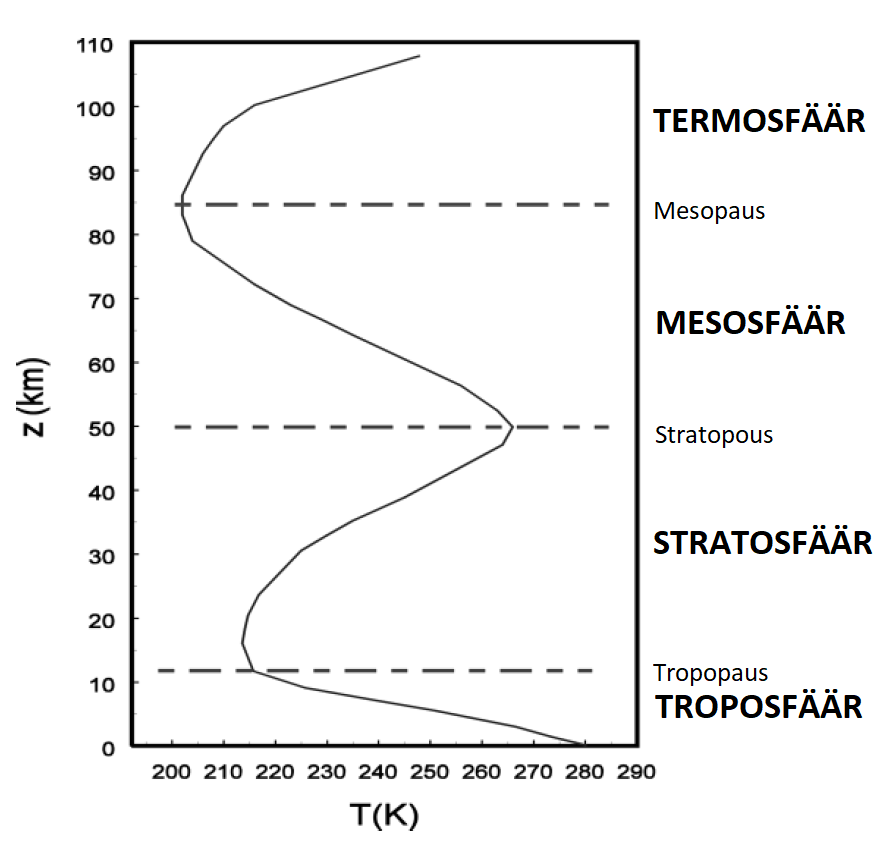
\includegraphics[width=0.5\textwidth]{Profile2.png}
	\caption{Temperatuuri sõltuvus kõrgusest}
	%\allikas{Minu programm}
	\label{profile}% Selle järgi viidatakse, see rida peab olema pärast \caption
\end{figure}

Joonisel \ref{profile} on näha, kuidas temperatuur muutub kõrguse kasvades. Troposfääris temperatuur langeb ja stratosfääris temperatuur tõuseb. Kõrguse kasvades rõhk väheneb, sest kõrguse kasvades väheneb ülevalpool oleva õhu mass, mis surub õhku kokku tekitades rõhku. Kuna rõhk väheneb, siis temperatuur langeb. See seletab temperatuuri langust troposfääris. Peale troposfääri tuleb osoonikiht, mis asub stratosfääris. Osoon neelab päikeselt tulevat kiirgust muutes selle soojuseks. Mida kõrgemal, seda vähem kiirgust on neelatud päikese poolt ja seda soojem. Eelkirjeldatud atmosfääri kihtides on kogutud käesoleva uurimistöö katseandmed.

Selles peatükis on avaldatud temperatuuri ja rõhu sõltuvused kõrgusest erinevate meetoditega, otsides kõige täpsemat seost.

Termodünaamika esimene seadus on avaldatud alljärgnevalt
\begin{equation}\label{eq1}
dU = dQ - dA
\end{equation}
kus $dU$ on gaasi siseenergia muutus, $dQ$ on soojushulga muutus ja $dA$ on töö muutus.

Gaasi siseenergia $U$ avaldub vabadusastmete $i$ kaudu järgneva seose abil
\begin{equation}\label{eq5}
U = \frac{i}{2} \nu R T
\end{equation}
Konstantse ruumala puhul tööd ei tehta, seega kogu soojus läheb siseenergia suurendamiseks. Saame soojusmahutavuse, võttes siseenergia muudust tuletise temeratuuri järgi.
\begin{equation}\label{eq6}
C_V = \frac{dQ}{dT}=\frac{i}{2}\nu R
\end{equation}
Molaarset soojusmahutavust saab avaldada valemiga $c_V = \frac{C_V}{\nu}$ saades molaarseks soojusmahutavuseks
\begin{equation}\label{eq7}
c_V = \frac{i}{2}R
\end{equation}

Kui aga vaadata isobaarilist protsessi, siis vaadates olekuvõrrandit tuleneb $pdV=\nu RdT$, ning gaas teeb tööd $dA = pdV = \nu RdT$. Avaldades need valemisse \ref{eq1} saame
\begin{equation*}
dQ = dU + dA = \frac{i+2}{2} \nu R dT
\end{equation*}
millest järeldub
\begin{equation*}
c_p=\frac{i+2}{2}R
\end{equation*}
Samuti saab näidata $c_V$ ja $c_p$ vahelist seost
\begin{equation}\label{eq9}
c_p = c_V + R
\end{equation}

Vaatame õhukest õhuriba laiusega $dz$ kõrgusel $z$. Rõhu muutust kõrguste $z$ ja $z + dz$ vahel saab kirjeldada valemiga
\begin{equation}\label{eq10}
dp=-\rho (z) gdz
\end{equation}
Kui seda integreerida, siis saab kätte rõhu muutuse sõltuvalt kõrgusest. Aga kuna tihedus ei ole konstantne, siis on vaja kõigepealt leida kuidas tihedus muutub kõrguse muutumisega.

\section{Ideaalne gaas}
Selles alampeatükkis teeme eelduse, et atmosfäär koosneb ideaalsest gaasist. Sellisel juhul saame kasutada ideaalse gaasi olekuvõrrandit
\begin{equation}\label{eq8}
PV=\nu RT
\end{equation}

\subsection{Isotermiline atmosfäär}
Oletame, et armosfääris on kõikjal ühtlane temperatuur. Sellisel juhul on atmosfäär isotermiline ja me saame asendada valemi \ref{eq8} valemise \ref{eq10} saades järgmise seose
\begin{equation}\label{eq16}
\frac{dp}{p} = -\frac{\mu g}{RT}dz
\end{equation}
Kuna temperatuur on konstantne, siis on ka $\frac{\mu g}{RT}$ konstantne ning seda integreerides saame järgneva
\begin{equation*}
\int_{p_0}^{p} \frac{dp}{p}  = \int_{0}^{z} -\frac{\mu g}{RT}dz
\end{equation*}
\begin{equation*}
\ln(\frac{p}{p_0}) = - \frac{\mu g}{RT} z
\end{equation*}
Kus $T$ on atmosfääri konstatntne temparatuur, $z$ on kõrgus maapinnalt, $p_0$ on kõrgus maapinnalt ja $p$ on rõhk kõrgusel $z$ maapinnast ja $p$ sõltub kõrgusest järgnevalt
\begin{equation*}
p = p_0 e^{-\frac{\mu g}{RT}z}
\end{equation*}
Kuid see valem ei kehti, sest atmosfääris pole ühtlane temperatuur.

          
\subsection{Adiabaatiline atmosfäär}
Adiabaatiline protsess on termodünaamiline protsess, mille käigus ei toimus soojusvahetust väliskeskkonnaga.

Harilikult on õhumassid atmosfääris tugevas liikumises, nii et nad liiguvad pidevalt üles-alla. Kuna kõrgemal on rõhk väiksem kui all, siis jahtub gaas üles liikudes adiabaatilise paisumise tõttu (õhumasside suurte mõõtmete tõttu on soojusjuhtivus hästi aeglane).

Kuna adiabaatilises protsessis soojusvahetust ei toimu, siis valemis \ref{eq1} $dQ=0$. Gaasi poolt tehtud töö on $d A=pdV$ ja gaasi siseenergia muut on $dU=\nu c_VdT$. Sellest järeldub
\begin{equation}\label{eq2}
\nu c_VdT = -pdV
\end{equation}
Ideaalse gaasi olekuvõrrandist \ref{eq8} saame tuletist võttes ja avaldades järgneva
\begin{equation}\label{eq3}
dT = \frac{pdV+Vdp}{\nu R}
\end{equation}
Asendades \ref{eq3} valemi valemisse \ref{eq2} saame uue seose
\begin{equation}\label{eq4}
pdV(c_V+R)+c_VVdp=0
\end{equation}
Asendame siia sisse valemi \ref{eq9} ja adiabaadi näitaja
\begin{equation*}
\gamma \equiv \frac{c_p}{c_V}
\end{equation*}
Nüüd eelmisi seoseid kasutades ja ümber paigudades saame võrrandi
\begin{equation*}
\gamma \frac{dV}{V} + \frac{dp}{p} = 0
\end{equation*}
Seda integreerides saame
\begin{equation*}
 \int \gamma \frac{dV}{V} + \frac{dp}{p} = \gamma \ln(V) + \ln(p) = Const.
\end{equation*}
Sellest saame järeldada
\begin{equation*}
pV^\gamma = Const.
\end{equation*}
Samuti kasutades ideaalse gaasi olekuvõrrandid saame tuletada veel 2 seost
\begin{equation}\label{eq13}
p^{1-\gamma}T^\gamma = Const.
\end{equation}
\begin{equation*}
V^{\gamma-1}T = Const.
\end{equation*}
Valemist \ref{eq13} saame
\begin{equation*}
d\ln(p^{1-\gamma}T^\gamma) = 0
\end{equation*}
Millest saame
\begin{equation}\label{eq17}
\frac{dp}{p} = \frac{\gamma}{\gamma-1}\frac{dT}{T}
\end{equation}
Võttes nüüd valemi \ref{eq16} ja valemi \ref{eq17}
\begin{equation*}
\frac{dT}{dz}=-\frac{\gamma-1}{\gamma} \frac{\mu g}{R}
\end{equation*}
Seda integreerides saame
\begin{equation*}
\int_{T_0}^{T} dT = \int_{0}^{z} -\frac{\gamma-1}{\gamma} \frac{\mu g}{R} dz
\end{equation*}
\begin{equation*}
T - T_0 = - \frac{\gamma - 1}{\gamma} \frac{\mu g}{R} z
\end{equation*}
Kus $T_0$ on temperatuur maapinnal ja $T$ on temperatuur kõrgusel $z$, mille saab avaldada sõltuvusena
\begin{equation*}
T=T_0 \bigg( 1-\frac{\gamma-1}{\gamma} \frac{\mu g}{R T_0} z \bigg)
\end{equation*}
Kasutades nuud seost \ref{eq13} saame seose
\begin{equation*}
p = p_0 \bigg( 1-\frac{\gamma-1}{\gamma} \frac{z}{z_0} \bigg)^\frac{\gamma}{\gamma-1}
\end{equation*}

\subsection{Mitteadiabaatiline atmosfäär}

\section{Wan der Waalsi gaasi mudel}
Wan der Waals esitas ideaalse gaasi olekuvõrrandist täpsema mudeli gaasi olekuvõrrandi jaoks.
\begin{equation}\label{eq15}
\nu RT = \bigg( p+\frac{\nu^2 a}{V^2} \bigg) \bigg( V - \nu b \bigg)
\end{equation}
Kus $a$ ja $b$ on igale  gaasile empiiriliselt määratud parameetrid. Siseenergia on antud kujul
\begin{equation}\label{eq14}
U = \nu c_VT-\frac{\nu^2 a}{V}
\end{equation}


\subsection{Adiabaatiline atmosfäär}
Siseenergia muutu saab avaldada valemist \ref{eq14}
\begin{equation*}
dU = \nu c_VdT + \frac{\nu^2 a}{V^2}dV
\end{equation*}
Adiabaatilise protsessi deffinitsiooni kohaselt ei anta gaasile siseenergiat juurde, ehk $dQ = 0$. Seega saame kirja panna
\begin{equation*}
0 = dU + pdV = \nu c_V dT + \bigg( \frac{\nu^2 a}{V^2} + p \bigg) dV
\end{equation*}
Asendades siia sisse valemi \ref{eq15} saame
\begin{equation*}
0 = c_V dT + \frac{RT}{V - \nu b}dV
\end{equation*}
\begin{equation*}
\int - \frac{c_V}{T} dT = \int \frac{R}{V - \nu b}dV
\end{equation*}
\begin{equation*}
c_V \ln(T) + R \ln(V - \nu b) = Const.
\end{equation*}
\begin{equation*}
(V - \nu b)^R T^{c_V} = Const.
\end{equation*}
\begin{equation*}
(V - \nu b)^{R + c_V} \bigg( p + \frac{\nu^2 a}{V^2} \bigg)^{c_V} = Const.
\end{equation*}
\begin{equation*}
 \bigg( p + \frac{\nu^2 a}{V^2} \bigg) (V - \nu b)^\gamma = Const.
\end{equation*}


\chapter{Katsed ja andmete analüüs}

Selle uurimistöö käigus tehti katse milleks oli heeliumõhupalliga andmete kogumine kogu lennu vältel. Heeliumõhupalli külge kinnitati sond, mis mõõtis õhurõhku, temperatuuri, õhuniiskust ja asukohta. Lend koraldati 10. veebruaril 2019.

Alguses oli plaanis lend teha väätsa staadionilt, aga kasutades http://predict.habhub.org/ lehel olevat kalkulaatorit oli ennustusest näha, et sond oleks kukkunud jõhvi lähedale. Kuna eksimusruum võib olla suur ning Venemaa piir ja meri pole kukkumis kohast kaugel otsustatti lennu start teha võimalikult edelast, nii et edela tuultega kalduks sond Kesk-Eestisse. Rihtides lõppsihtkohta Paide peale otsustatti start teha Varblast, Pärnumaalt.

Sondi sees olev ruum oli jaotatud kaheks. Alumises olid kaks toru mis olid parralleelsed ja läbisid sondi kere. Nenede sees olid klappid, ventilaator ja filtrid. Selle eesmärgiks oli koguda tolmu ja muud, mis jääb filtrisse kinni kõrgemal kui 20km. Teatud kõrguse saavutamisel pöörab raspbarry Pi mootori \SI{90}{\degree} päripäeva avades nii klappid ja sulgedes lüliti. mille tõttu hakkavad ventilaarotid tööle. Kui võrgus on vähenenud soovitud kõrgusest siis pöörab raspbarry Pi mootori algasendisse. Sulgedes sellega klappid ja ühendades ventilaarotid vooluringist lahti. Tolmu kogumine ei käi selle uurimistöö juurde.

\begin{figure}[h]
	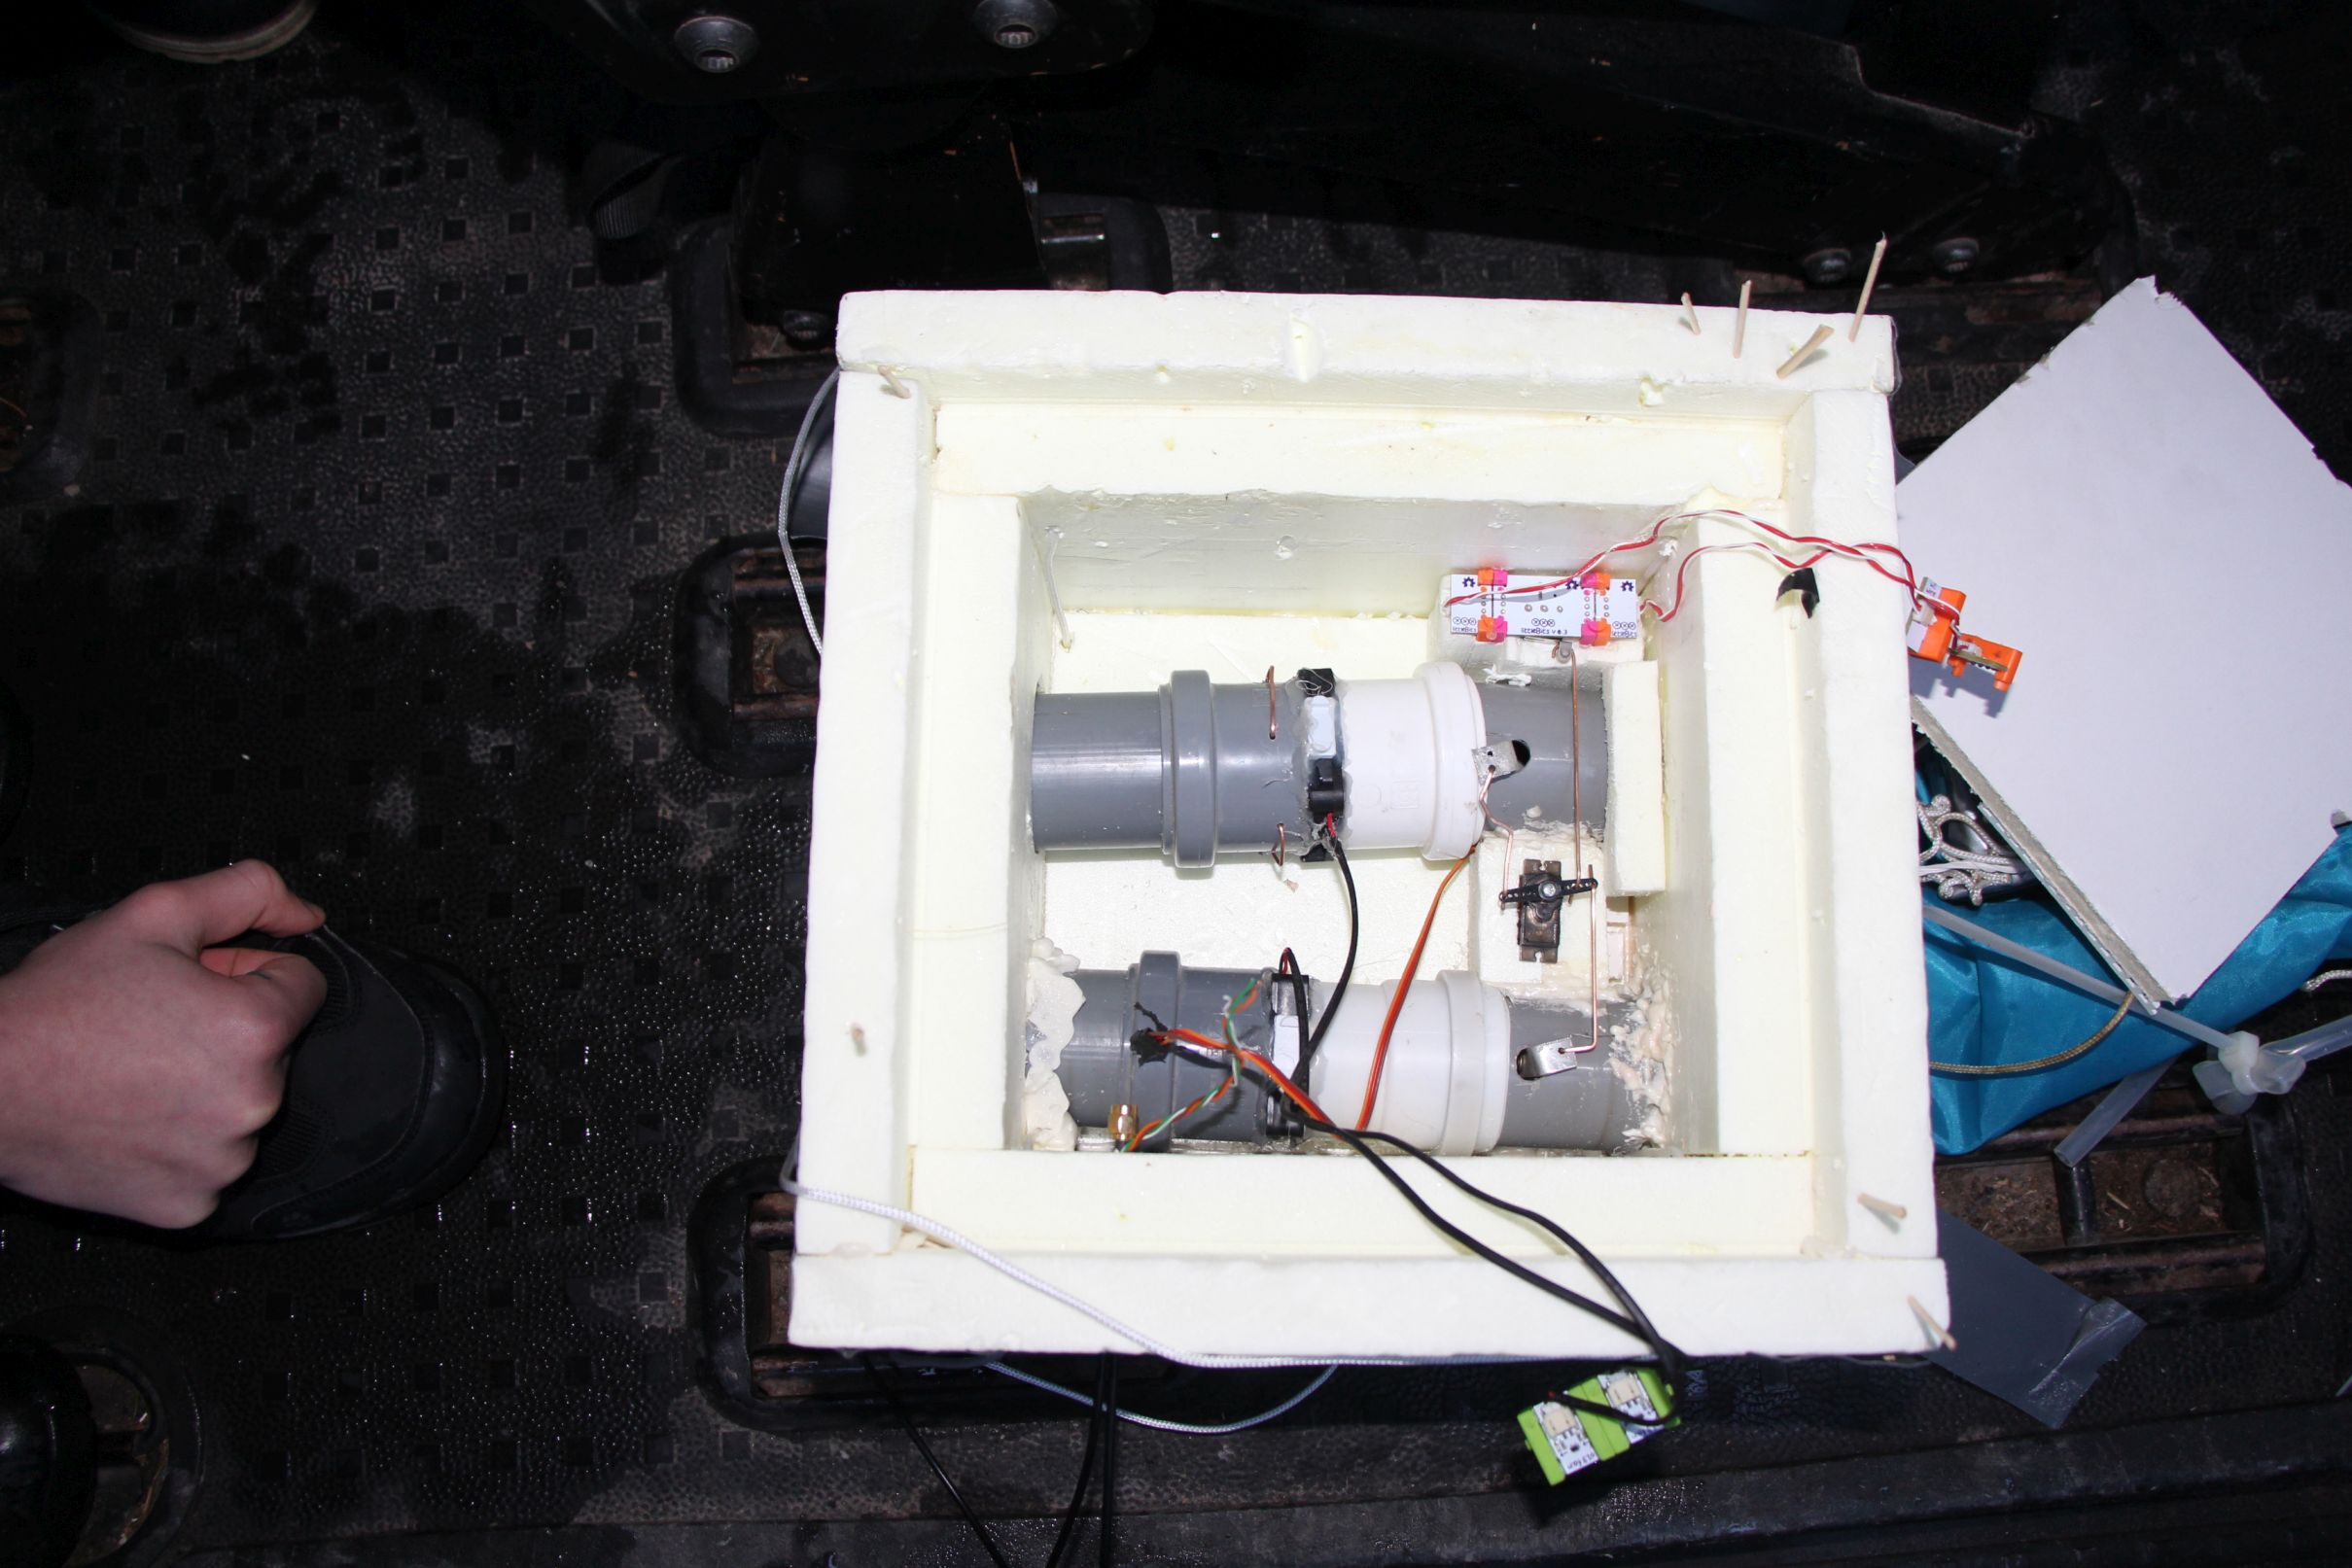
\includegraphics[width=0.5\textwidth]{PicGra/sond2korrus.jpg}
	\caption{Pilt sondist}
	\allikas{\url{http://pildid.real.edu.ee/main.php?g2_itemId=84949}}
	\label{sond}% Selle järgi viidatakse, see rida peab olema pärast \caption
\end{figure}

Ülemises osas oli kogu tehnika. Mõõtmisi tegi ja klappe avas Raspberry Pi arvuti. Voolu andis nii ventilaatoritele kui ka Raspberry Pi'le akkupank. Raspberry Pi külge oli kinnitatud raadio antenn, Gps antenn mootor klappide jaoks ja andur BME280 mis mõõtis väljas olevat rõhku, temperatuuri ja õhuniiskust.

\begin{figure}[h]
	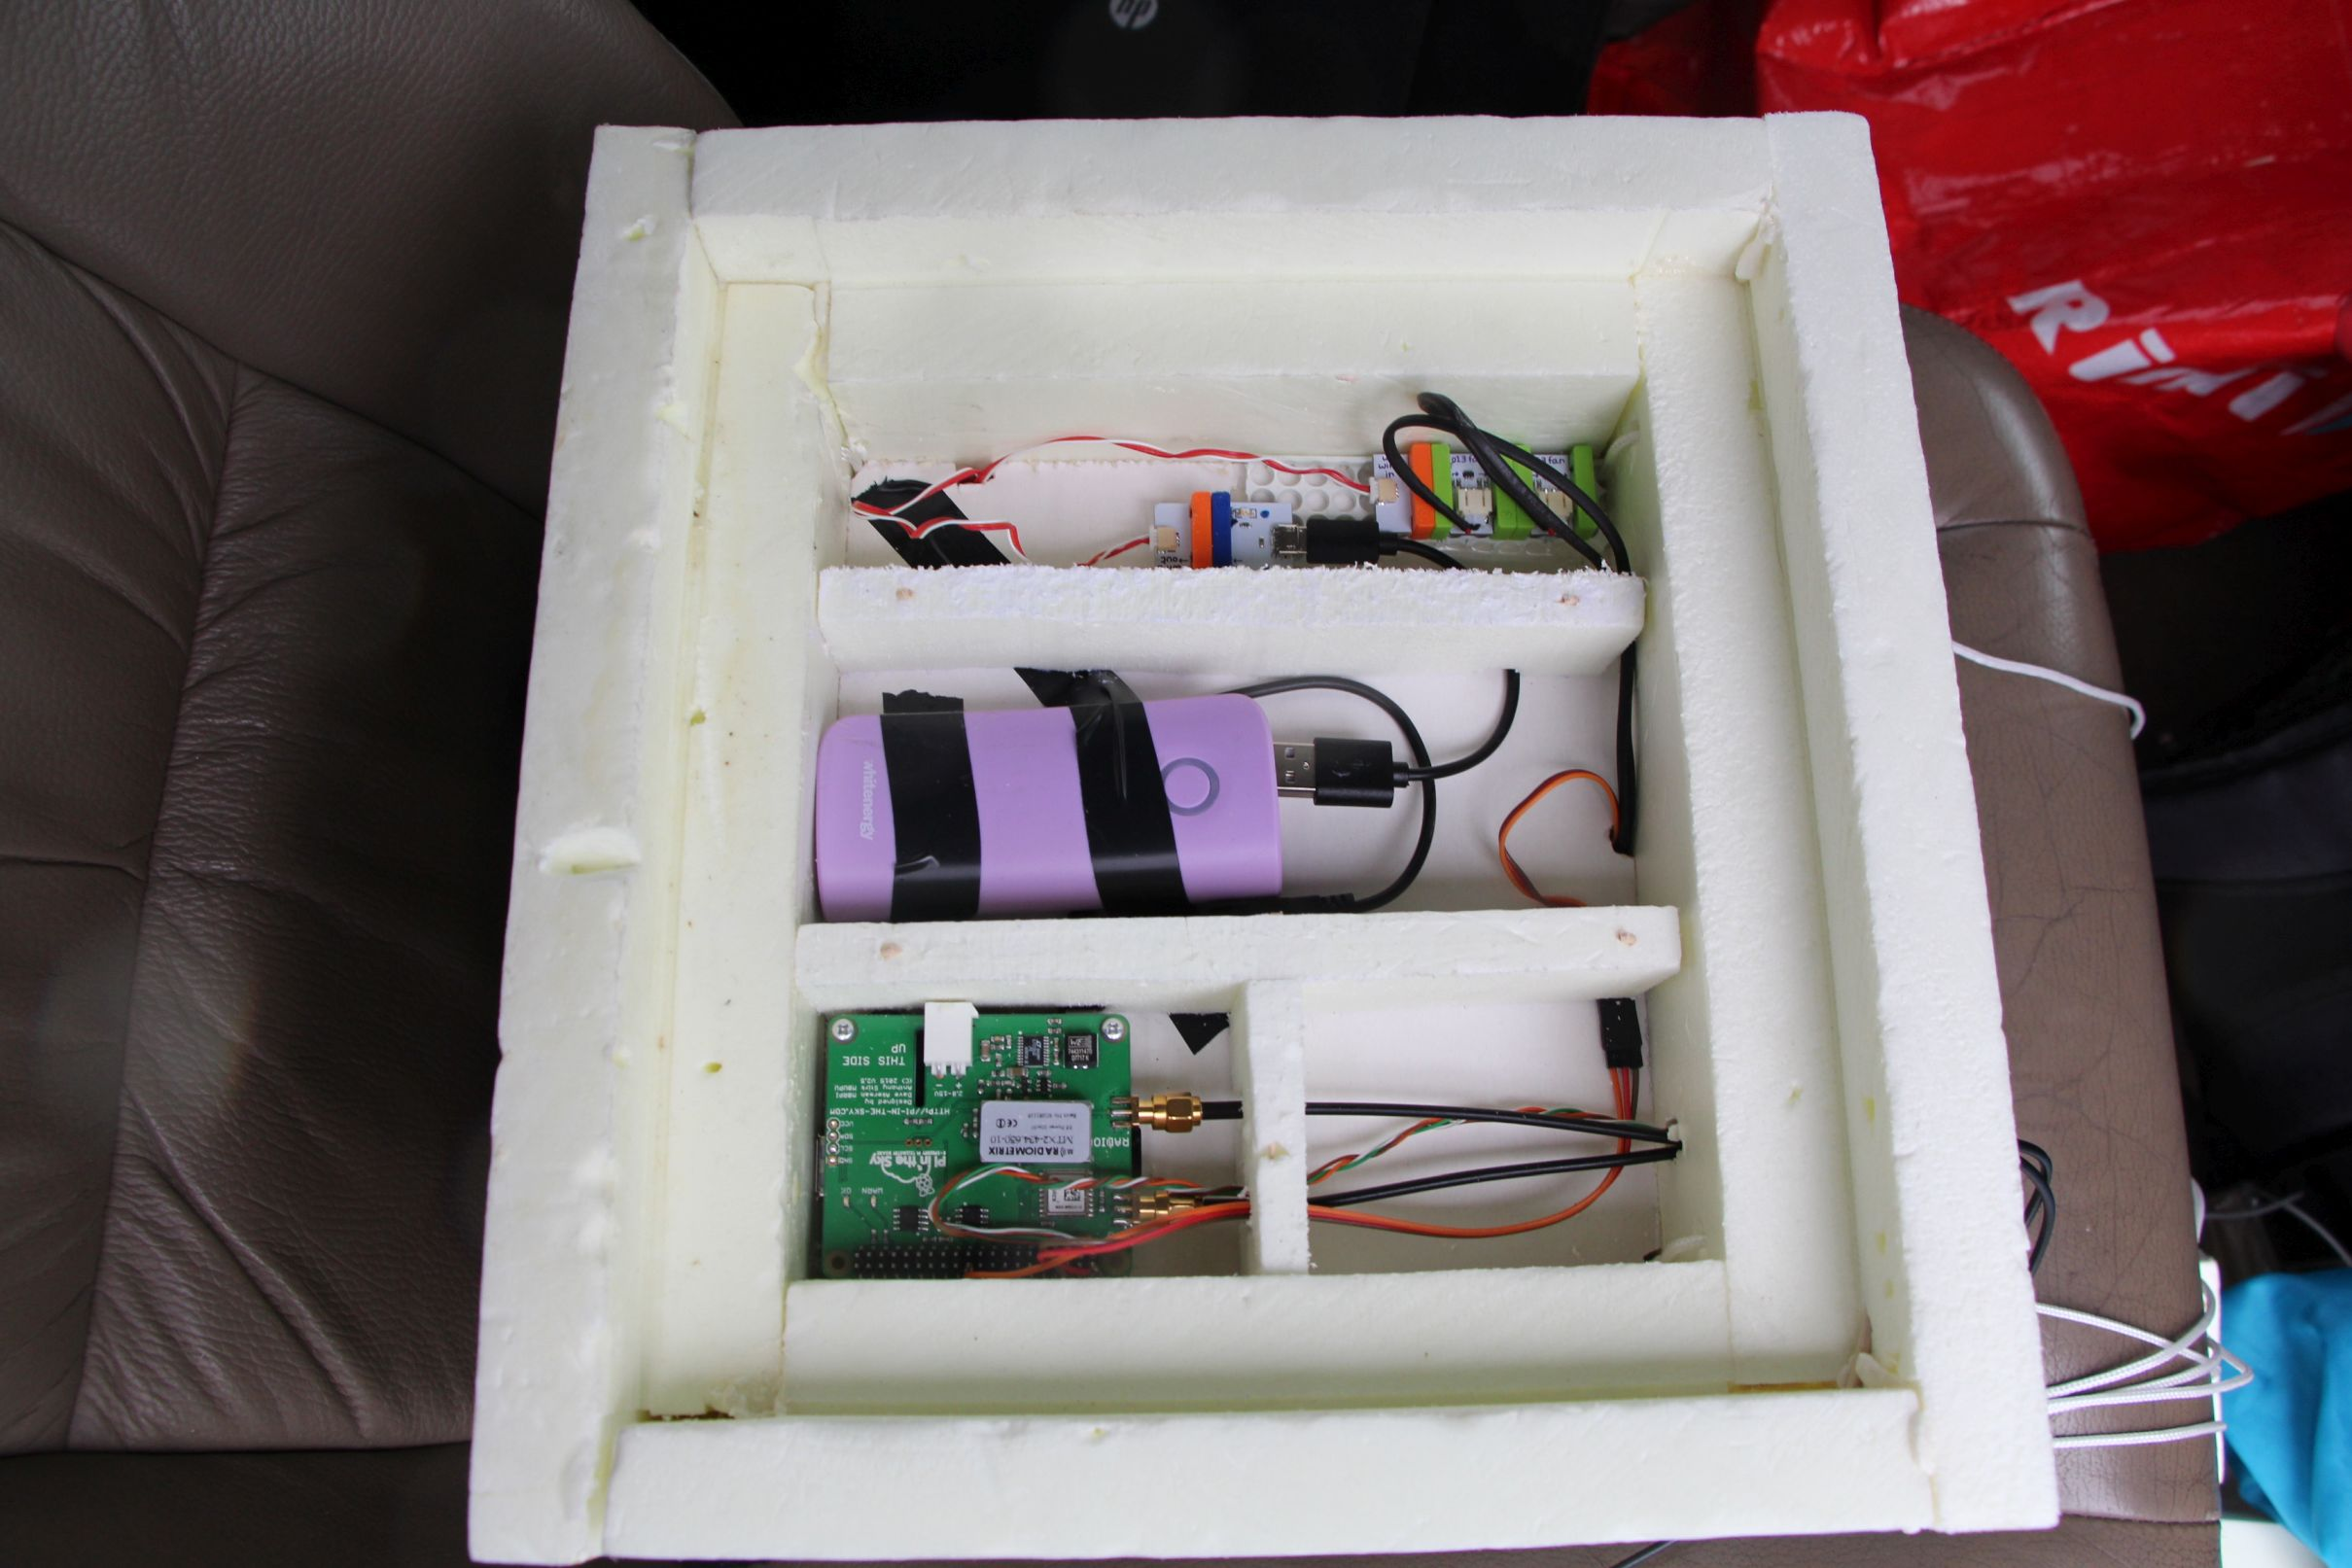
\includegraphics[width=0.5\textwidth]{PicGra/sond1korrus1.jpg}
	\caption{Pilt sondist}
	\allikas{\url{http://pildid.real.edu.ee/main.php?g2_itemId=84949}}
	\label{sond}% Selle järgi viidatakse, see rida peab olema pärast \caption
\end{figure}

Sondi mass oli \SI{1375}{g}. Sondi korpus oli ehitatud kasutades penoplasti ja puit tikke. Sondist tuli välja nii raadio kui ka GPS antenn, ning ka andur BME280. Sondi peale oli kinnitatud langevari. Eraldi korpuses asus GPS tracker GL370?? mida kasutatti pärast sondi leidmisel. Lennuks kasutatti Hwoyee \SI{600}{g} õhupalli. Sinna sisse lasti umbes 2800 l heeliumi.

\begin{figure}[h]
	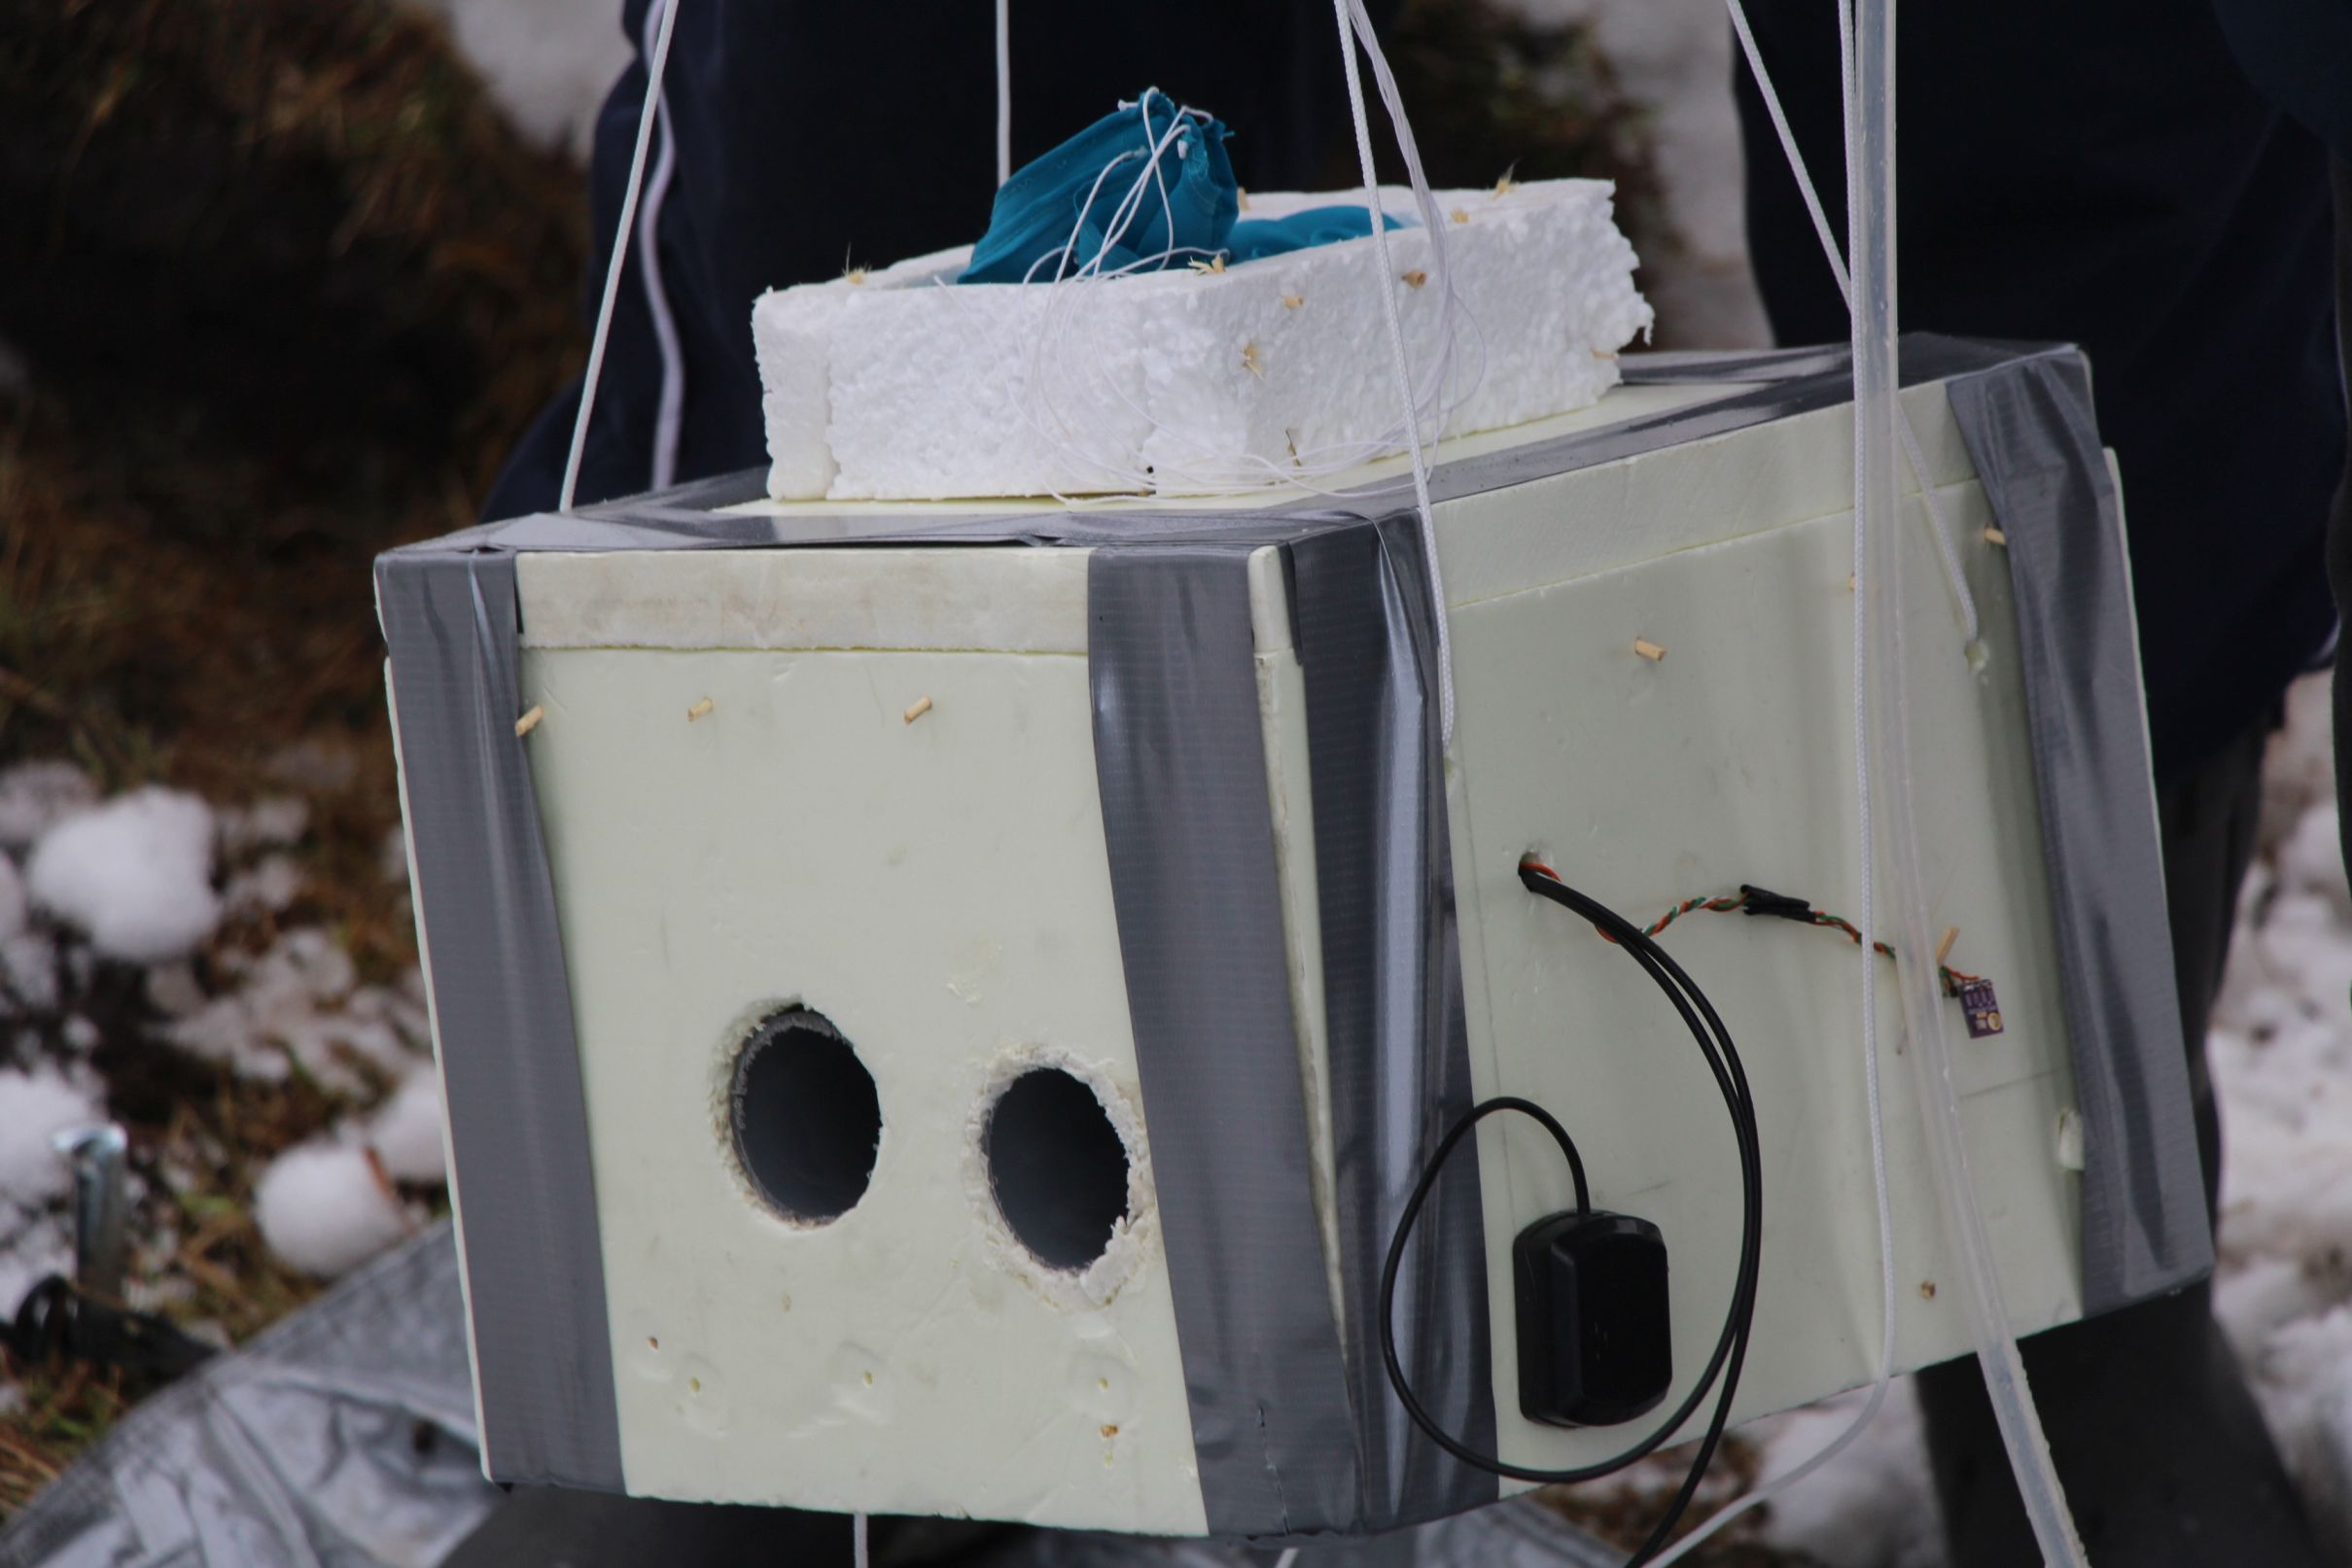
\includegraphics[width=0.5\textwidth]{PicGra/sond.jpg}
	\caption{Pilt sondist}
	\allikas{\url{http://pildid.real.edu.ee/main.php?g2_itemId=84949}}
	\label{sond}% Selle järgi viidatakse, see rida peab olema pärast \caption
\end{figure}

Lennu start oli kell 11:51. Algul saadi andmeid kätte raadio teel saadetud signaalist. Raadioside töötas umbes 20 min. Peale seda polnud võimalik puhast signaali kätte saada. Siis kadus GPS trackeri ühendus mobiilisideme teenuspakkujaga kõrguse pärast. Peale maandumist ühendas GPS Tracker ennast uuesti teenusepakkuja võrku ja saadi teada sondi kukkumise asukoht. Sond maandus Paide lähedal paarkümmend meetrit Tallinn-Tartu maanteest. Lend lõppes kell 14:06. Siis saime sondi kätta ja lugesime Raspberry Pi poolt tehtud logiandmed maha.

\section{Metoodika}
\subsection{Andmete kogumine}
Andmeid kogutakse heeliumiga täidetud õhupalliga kaasa saadetud sondiga, mis mõõdab erinevaid andmeid. Põhilisteks andmeteks on kõrgus, asukoht, aeg, välistemperatuur ja rõhk. Sondi pardal on Raspberry Pi arvuti. Õhupall kerkib atmosfääri kõrgemadesse kihtidesse, sest üleslükkejõud ületab kerge gaasi ja sondi massi. Kõrgemale tõustes rõhk väheneb. Et õhupalli siserõhk oleks tasakaalus välisrõhuga, suureneb õhupalli ruumala, kuni õhupall lõhkeb ülepingest. Peale seda kukkub sond alla ja leitakse GPS'ga üles.
\subsection{Andmete analüüs}
Andmete analüüsimisks kasutan enda poolt kirjutatud c++/Python programmi. Programmiga saab joonistada graafikuid andmete põhjal ja kontrollida erinevaid seoseid.

\section{Varem tehtud katsed}
Selles uurimistöös tehtud katsed on tehtud Eesti kosmosekoolide võrgustiku siseselt. See võrgustik on varem teinud juba kaks heeliumõhupalli lendu, ning selle uurimistööga seoses tehakse ka heeliumõhupalliga lend. Uue katse planeerimiseks on vajalik eelmiste katsete analüüs ja leida vigu, mida uues katses parandada.
\newline Esimene lend mis tehti 29. märtsil kestis umbes kaks tundi, kus kõrgeim punkt milleni jõuti oli 26474 m. Selleks läks aega poolteist tundi ja sellel kõrgusel lõhkes õhupall väikese välisrõhu pärast suureks paisumise tõttu. Kokku tehti 220 mõõtmist. Mõõtmise alla kuulusid kellaaeg, laiuskraad, pikkuskraad, kõrgus, kapsli sisetemperatuur, välistemperatuur ja rõhk.
\newline Teine lend tehti 11. mail ning seekord kestis lend peaaegu neli tundi, jõudes kolme ja poole tunniga kõrgusele 32608 m. Katse tegijad muutsid õhupallis heeliumi kogust, mille tõttu oli tõusmise kiirus väiksem, aga õhupall plahvatas hiljem ja jõuti kõrgemale. Seekord tehti 4300 mõõtmist ja mõõdeti samu parameetreid.
\newline Ma kasutan teise lennu andmeid, et planeerida enda lendu, sest teisel lennul on tihedamad andmepunktid.

\subsection{Kõrguse sõltuvus lennuajast}
Joonisel \ref{NK_H_T} on näha õhupalli kõrgust lennu jooksul muutuvana ajast. Kuna mõõtmised on tehtud kindlate ajavahemike tagant on näha, kuidas peale õhupalli lõhkemist langeb sond kiiremini ja hakkab peale seda aeglustama. %(huvitav, kuidas õhupall läheb koguaeg ühtlase kiirusega ülesse(Jarl mõtle hiljem üle)).


\begin{figure}[h]
	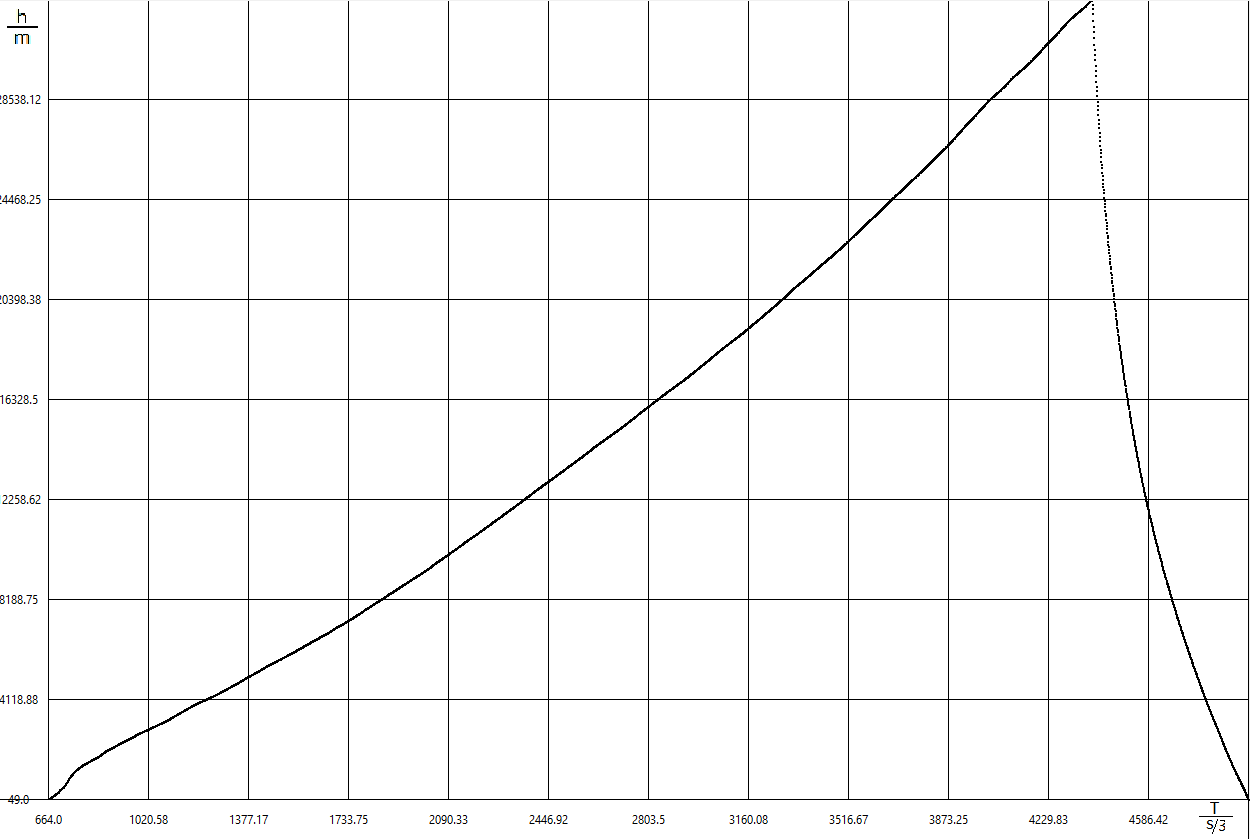
\includegraphics[width=1\textwidth]{NK_H_T.png}
	\caption{Kõrguse sõltuvus ajast}
	%\allikas{Minu programm}
	\label{NK_H_T}% Selle järgi viidatakse, see rida peab olema pärast \caption
\end{figure}


\subsection{Rõhu sõltuvus kõrgusest}
Joonisel \ref{NK_R_H} on näha rõhu sõltuvust kõrgusest. Graafikult tuleb ilusasti välja sõltuvus, välja arvatud umbes 10 km kõrgusel, kus jookseb kaks joont. Erinevus tekib, sest üks joon näitab andmeid tõusmisel ja teine langemisel.
\begin{figure}[h]
	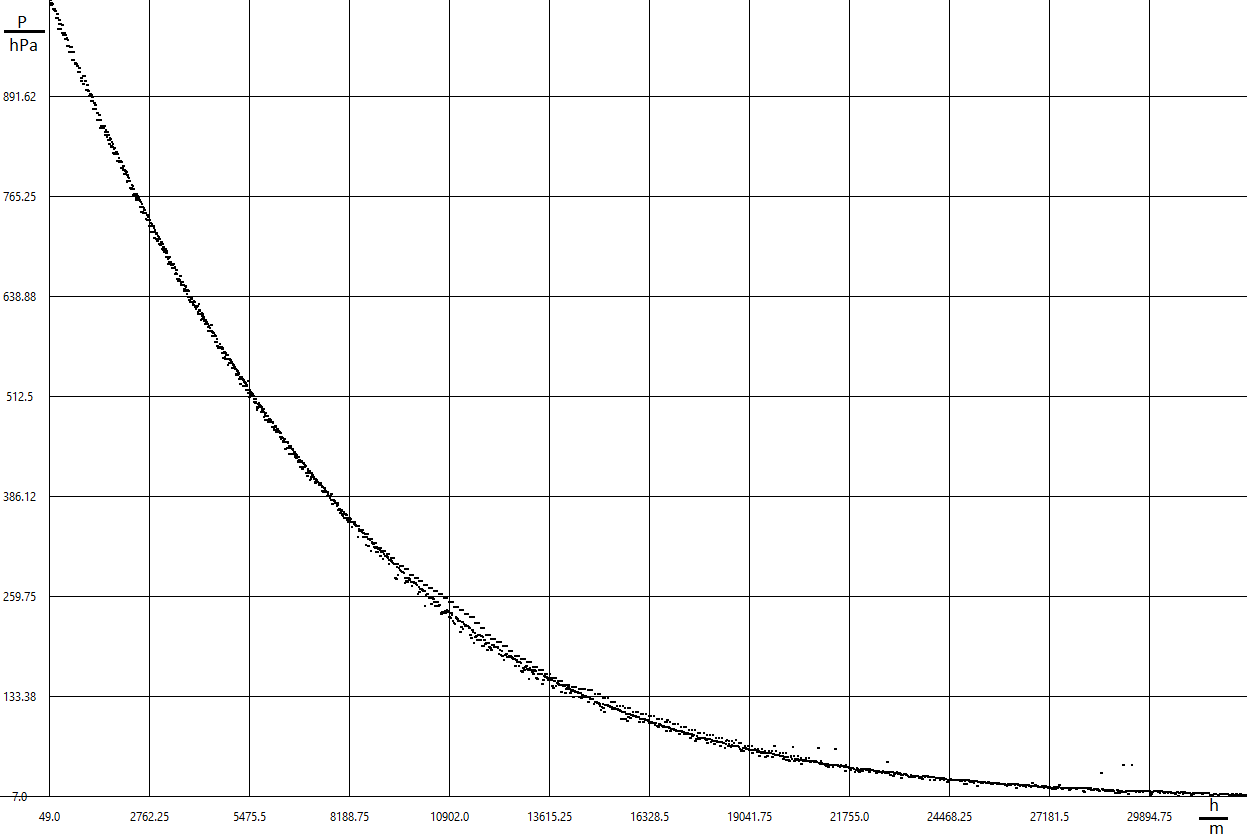
\includegraphics[width=1\textwidth]{NK_R_H.png}
	\caption{Rõhu sõltuvus kõrgusest}
	%\allikas{Minu programm}
	\label{NK_R_H}% Selle järgi viidatakse, see rida peab olema pärast \caption
\end{figure}

\subsection{Välistemperatuuri sõltuvus kõrgusest}
Joonisel \ref{NK_T_H} on näha välistemperatuuri sõltuvus kõrgusest. Nagu  joonisel \ref{NK_R_H} on ka siin näha kahte joont, mis tuleb tõusmisest ja langemisest. Tõusmisel on andmepunktid väga laiali valgunud, mis tuleb sondi pöörlemisest. Vahepeal on temperatuuri andur päikese poole, mille tõttu temperatuur on suurem ja vahepeal on andur päikesest eemal, mis juhul mõõdetakse tegelikku temperatuuri. Langemisel on pöörlemist vähem ja siis on punktid rohkem ühe joone peal. Et enda katses vältida andmete laialivalgumit, on vaja lahendada päikesest tulenevat temperatuur väärmõõtmise probleemi.
\newline On näha, et temperatuur ei lange pidevalt atmosfääris tõustes. Troposfääris temperatuur langeb, kuid strarosfääri jõudes hakkab temperatuur tõusma. Kõige külmem piirkond umbes 10 km kõrgusel.
\begin{figure}[h]
	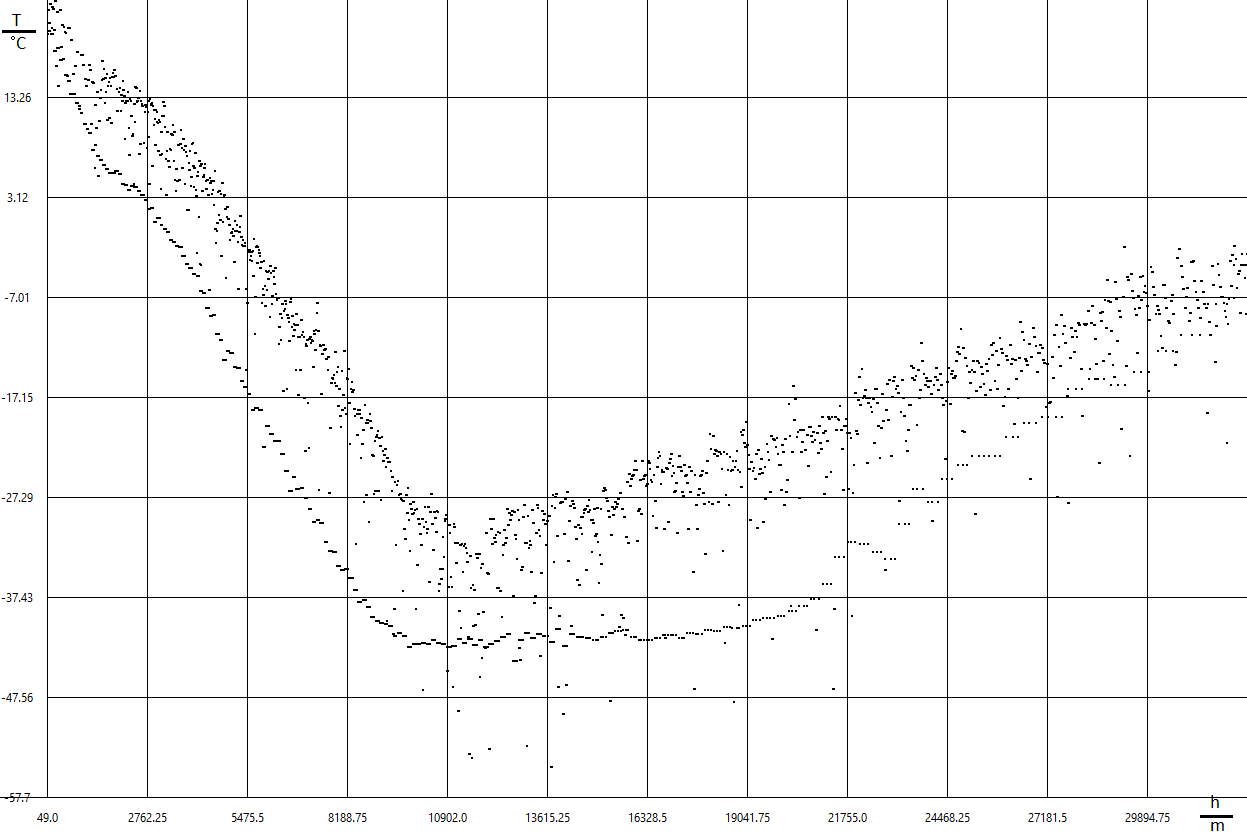
\includegraphics[width=1\textwidth]{NK_T_H.png}
	\caption{Välistemperatuuri sõltuvus kõrgusest}
	%\allikas{Minu programm}
	\label{NK_T_H}% Selle järgi viidatakse, see rida peab olema pärast \caption
\end{figure}


 
\addchap{Kasutatud materjalid}% Viitamine paraneb veel

Hobbs, P. V., Wallace, J. M. (2006) Atmospheric Science: An Introductory Survey. Amsterdam: Elsevier \newline
Ahrens, C. D., Henson, R. (2018) Meteorology Today: An Introduction to Weather, Climate, and the Environment. Boston: Cengage Learning

%\cite{examplebook}% Kõige lihtsam viitamise käsk 
%\cite{examplearticle}
%\cite{exampleonline}

%\printbibliography% Selle käsuga trükime kasutatud materjalid, kommenteeri see kiirema kompileerimise jaoks

%\appendix% Lisad
%\chapter{Kes see lisatööd ikka teha tahab}% Lisa pealkiri

\kinnitusleht% Kinnitusleht
\end{document}
